\section{Packing Compiler \rr}
The \lan compiler is written in \texttt{Haskell} using the \texttt{cabal} packaging system
\cite{cabal}. Therefore, the \texttt{.cabal} file located in the root of the package, indicate
the structure of the program. The structure of the program can be seen in figure
\ref{fig:structure}. It consists of $3352$ lines of \texttt{Haskell} code, $197$ lines of
bash code, and some \texttt{html}, \texttt{PHP}, \texttt{css}, and \texttt{javascript}.

\begin{figure}[H]
    \centering
    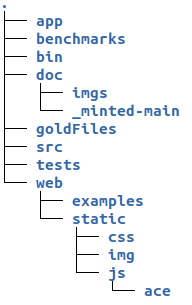
\includegraphics[scale=0.7]{imgs/directory-structure.png}
    \caption{Directory hierarchy of \lan package, printed out using \lsin{tree}.}
    \label{fig:structure}
\end{figure}
\noindent
The directory hierarchy holds the following purpose:

\begin{itemize}
    \item The \texttt{src/} folder contains the \lan library code, and \texttt{app/} contains a
          simple executable of the compiler. This division is used, in order to allow other
          packages to import and use different parts of the \lan compiler.

    \item \texttt{benchmarks/} contains the benchmark
          programs, the \texttt{cabal} benchmark file \texttt{HaskellBenchmark.hs}, and the
          \texttt{bash} script handling the execution time benchmarks.
    
    \item \texttt{bin/} contains the \lan executable and the \texttt{bash} test script.

    \item \texttt{doc/} contains the \LaTeX ~source files for this report.

    \item \texttt{goldFiles/} contains all the gold files used during testing, and
          \texttt{tests/} contains all the \lan test files.

    \item \texttt{web/} contains the source code for the \lan playground webpage. Within this
          directory \texttt{examples/} contains the example programs used in the playground,
          \texttt{static/} holds all the \texttt{javascript}, \texttt{css}, and images
          used for the interface. \texttt{web/} itself holds the \texttt{PHP} scripts
          handling the communication between the web page and the underlying server;
          meaning calling the \lan compiler and loading example programs.
\end{itemize}

\subsection{Compiler Package and Usage \rr}
% Installation, requirements, usage
As before mentioned the \lan package is created using \texttt{cabal}. Hence it can be constructed
using the regular \texttt{cabal} commands.
In order to build the compiler, \texttt{cabal} version $2.4$ is required. To install the
required dependencies issue the \texttt{cabal install} command.
A \texttt{Makefile} is included within
the root directory, that contains commands for 1) building the compiler, 2) testing the compiler
3) benchmarking the compiler. To perform these functions simply issue the commands below from
the root directory:
\begin{enumerate}
    \item \texttt{make}
    \item \texttt{make test}
    \item \texttt{make bench} or \texttt{make benchR}
\end{enumerate}
\noindent
All of the above will build the compiler anew, and create an executable \texttt{japa} in the
\texttt{bin/} directory.
\\
\\
The web-based \lan playground can be run using \texttt{PHP}. To boot up a local web server,
navigate to the \texttt{web/} directory and run:
$$\texttt{php -S localhost:<port number>}$$
\noindent
This will start a process running the web server on your localhost IP, on port $<port number>$.
Now simply navigate to a browser, and paste \texttt{localhost:<port number>} into the search bar,
and you will be taken to the webpage.

\subsection{Web Interface for Compiler \rr}
The web interface is based upon that of the \texttt{Janus} playground \cite{janusInterp} from
the bachelor thesis written by Claus Skou Nielsen and Michael Budde \cite{janusPlayground}.
The code has merely been altered to fit the purpose of the \lan showcase. Hence the only
modifications are within:

\begin{itemize}
    \item \texttt{index.html} to split the window vertically instead of horizontally,
          because the purpose of the webpage is to showcase the output \texttt{C++}
          code, and not interactively write \lan code. Some buttons has also been
          removed or altered.

    \item \texttt{execute.php} to not run an interpreter, but to run the \lan compiler
          on the input program in the playground.

    \item \texttt{playground.js} to follow the new format and functionality of the playground.

    \item \texttt{playground.css} to make the \texttt{css} match the new functionality with
          the vertical split.

    \item \texttt{mode-janus.js} to make syntax highlighting match \lan and not
          \texttt{Janus} syntax.
\end{itemize}
\noindent
It is indicated in each file, what has been created for this project, by outlining them
in comments such as:
\begin{lstlisting}
///////////////////////////////   "new"  //////////////////////////
some code
////////////////////////////// "new" end //////////////////////////
\end{lstlisting}
\noindent
An image of the \lan playground can be seen in figure \ref{fig:japa-playground}.
The left pane view is a textarea that takes in the \lan program. The right pane view
displays the compiled \texttt{C++} code. To compile a \lan program simply insert the program
in the left view, press the green button that says \texttt{C++}, and wait for it to show
in the right pane. A small number of example programs, has been pre-written and can be inserted
using the \texttt{Example} dropdown. The \texttt{About} page simply states where most of the
source code is taken from, and that it has been adapted to the need of this project.

\begin{figure}[H]
    \centering
    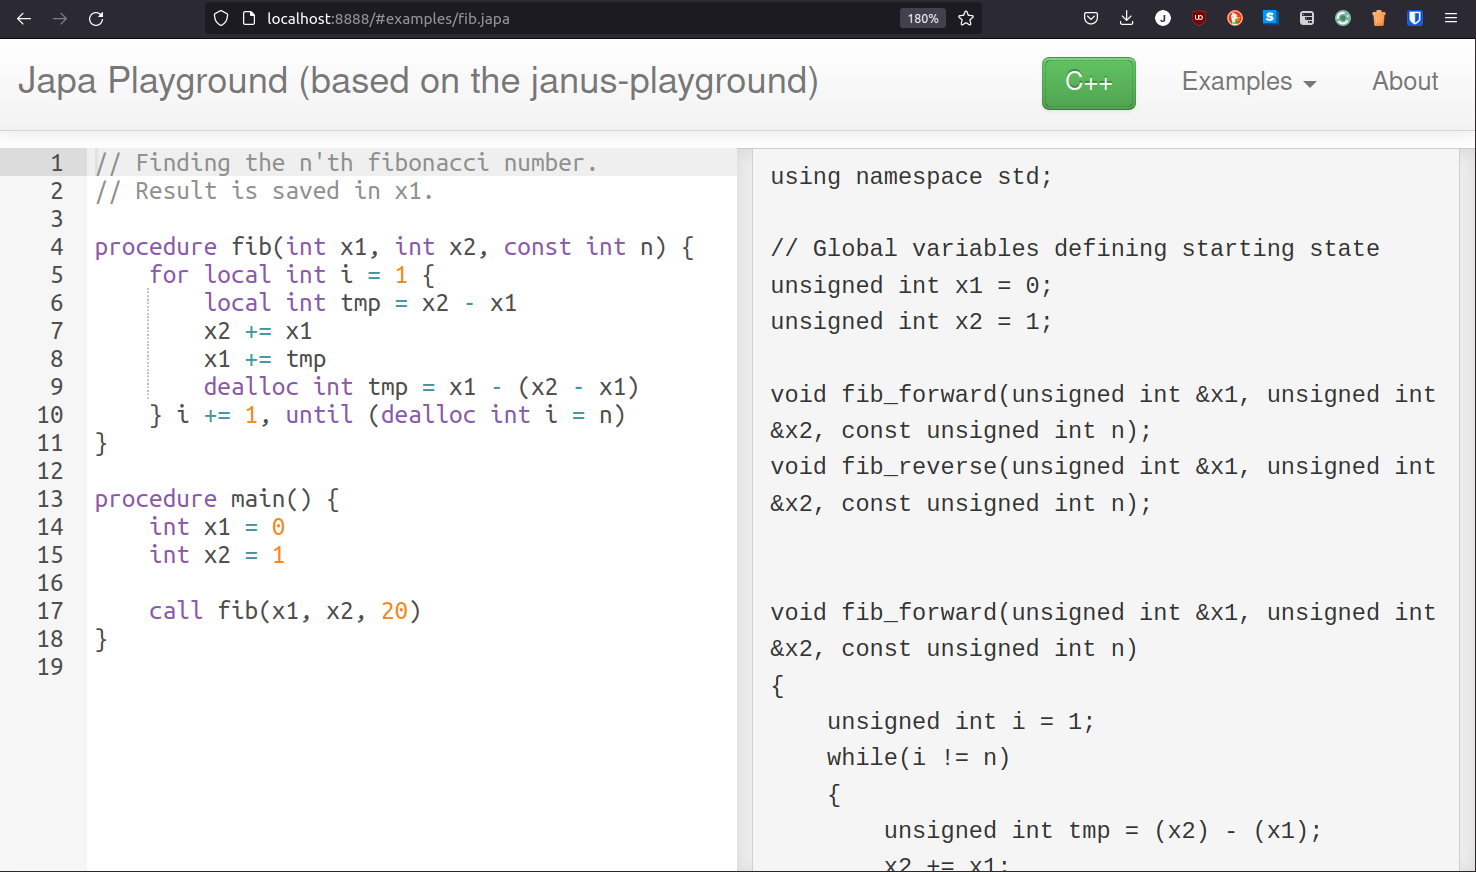
\includegraphics[width=\textwidth]{imgs/japa-playground.png}
    \caption{\lan playground allowing to write and translate \lan code to \texttt{C++}}
    \label{fig:japa-playground}
\end{figure}